\section{Evaluation}
\label{sec:evaluation}

To measure the performance impact of metadata tracking,
we instrumented all the SPECint2006~\cite{henning2006spec} applications to observe the
overhead it introduces. As a baseline, we compiled the applications with
SafeStack enabled since it is advertised as a viable replacement for stack
canaries, even showing lower overhead on some benchmarks~\cite{kuznetsov2014cpi}.
We also use tcmalloc as the heap allocator for our baseline, as it can have
very different run-time performance compared to the system allocator. This decision
is also motivated by the fact that we observed a 5\% improvement of execution
times when using tcmalloc on SPECint2006 (geometric mean). This improvement
increases to 20\% when considering only the C++ benchmarks. The machine used for these
experiments has a Xeon 5620 CPU running Ubuntu 12.04 64-bits.
\looseness=-1

Figure~\ref{fig:spec} shows the overhead introduced with the different configurations
of \projectname{}. We evaluated creating and initializing both 1 and 8-bytes of metadata
for all objects. These setups correspond to different instrumentation types,
like write integrity tracking or type hashes.
The overhead numbers are very low, with the maximum being around 15\% for perlbench and
the geometric mean being $<2$\% for both setups (1.2\% for one byte and 1.5\% for eight bytes). The results also show that metadata size has a
limited impact on the overall performance, showing that the variable compression ratio can help
deal with applications requiring complex metadata. While the measured overhead only includes
the metadata creation and initialization, not the instrumentation itself,
the latter can be tuned with careful design and is the topic
of future work using \projectname{}. To compare \projectname{} against existing metadata tracking
systems, we also implemented and evaluated the metadata shadowing scheme proposed by 
Akritidis et al.~\cite{akritidis2008preventing}. This approach shadows every group of 8
data bytes with a single metadata byte residing within an array allocated at a fixed location.
Even this simple shadowing scheme results in a significantly larger overhead as shown on Figure~\ref{fig:spec}.
The overhead for perlbench explodes to 70\% (going out of bounds in the figure) and the geometric mean across
all benchmarks increases to more than 8\%.

\begin{figure}[t]
\center
  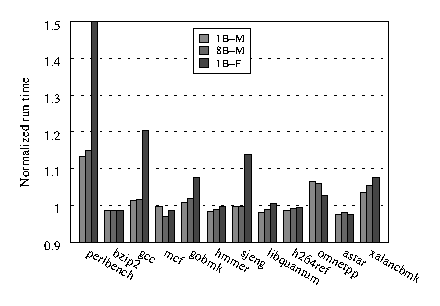
\includegraphics[width=2.8in]{plots/bargraph_runtime_spec.eps}
  \caption{
  SPECint2006 overhead with different configurations of \projectname{}. 1(8)B-M represents the configuration with
  1(8)-byte metadata entries. 1B-F represents the fixed compression ratio metadata shadowing from WIT~\cite{akritidis2008preventing}.
  }
  \label{fig:spec}
  \vspace{-1em}
\end{figure}
